\documentclass[10pt]{article}
\usepackage{amsmath}
\usepackage{listings}
\usepackage{graphicx}
\graphicspath{ {./images/} }
\begin{document}
{\centering
    CSU44061 Machine Learning - Week 2
    \par
    Samuel Petit - 17333946
    \par
    Dataset \# id:9--9--9 
    \par
}
\section*{Question a}
Code for all questions provided in the appendix.
\subsection*{Part i}

Using matplotlib with python to generate graphs, I plotted X2 against X1 (both features)
and made the colour of the marker different based on the prediction.
The red colour represents a positive prediction (+1) and the blue colour represents a negative
prediction (-1)

\vspace{5mm} %5mm vertical space

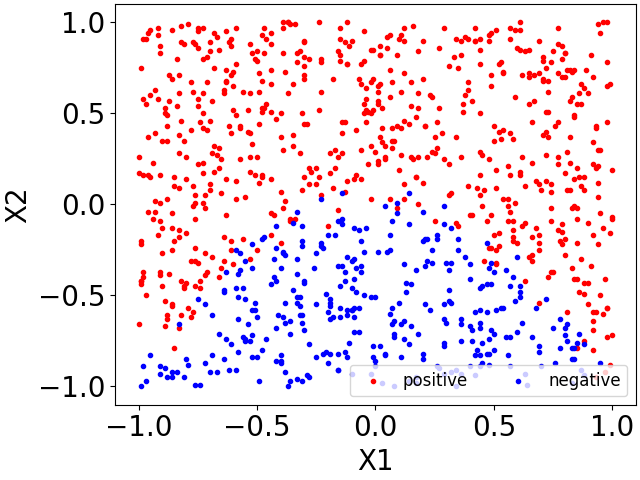
\includegraphics[scale=0.35]{Figure_1.png}

\subsection*{Part ii}
Using code provided in the appendix, I trained a logistic regression
classifier which gave me the following model:

\begin{equation*}
    \theta_{0} + \theta_{1}x_{1} + \theta_{2}x_{2} = -1.91100581 - 0.18987022 * x_{1} - 5.76650534 * x_{2}
\end{equation*}

\subsection*{Part iii}
The following plot plots X1 against X2, using the predictions and
the actual y output from the dataset.
the y output and predictions use different colours and markers to attempt to marke
this graph more readible.



It is a bit hard to see however we can clearly see that the predictions
are quite rough and very inacurrate on the edges as well as the top of the
slope.

As for the slope representing the classifier separation, I used the
following equation. It is obtained by computing the sum of the linear function
which uses $\theta_{0}$ and $\theta_{1}$ and dividing the result
by the 3rd value of the model: $\theta_{2}$.

\begin{equation*}
    y = -\frac{\theta_{1} * x_{1}^{i} + \theta_{0}}{\theta_{2}}
\end{equation*}

\vspace{5mm} %5mm vertical space

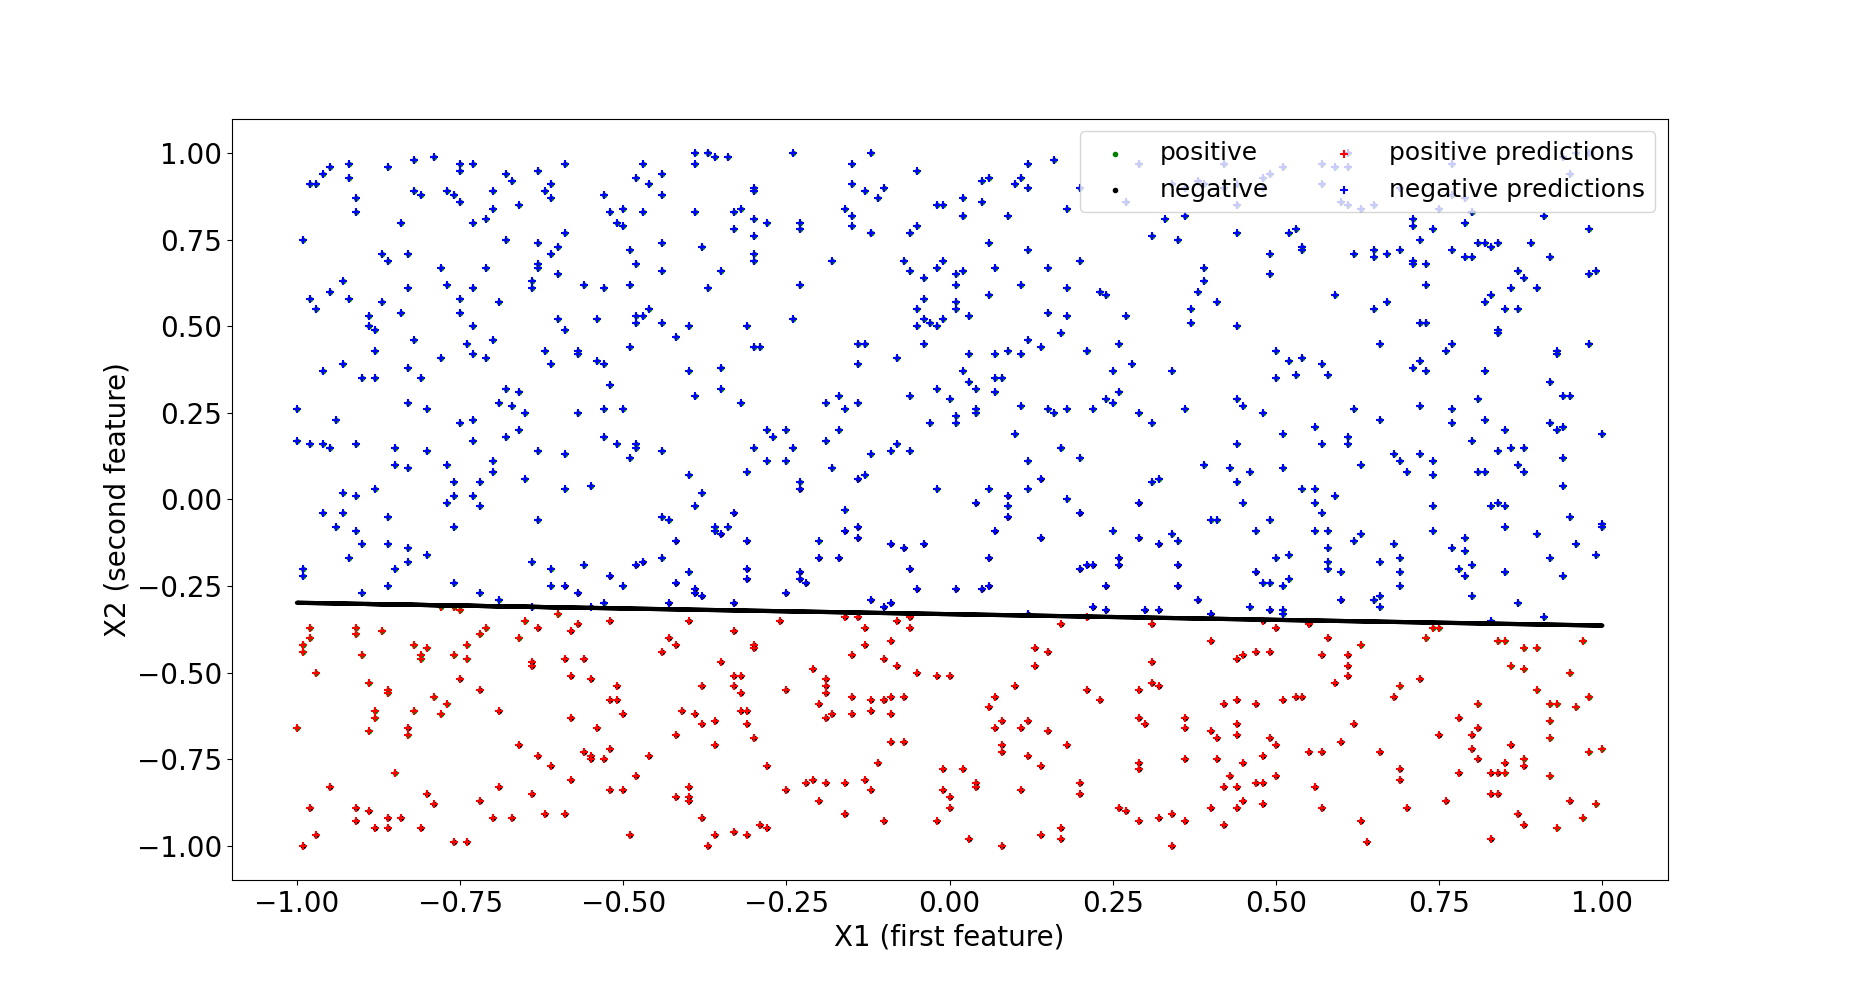
\includegraphics[scale=0.245]{Figure_2.png}

\section*{Question b}
\subsection*{Part i}
Using code provided in the appendix, I trained a linear SVM
classifier with 3 different C values. I obtained the following parameters:

C = 0.001
\begin{equation*}
    -0.21517665 - 0.00849777 * x_{1} - 0.47908454 * x_{2}
\end{equation*}

C = 1
\begin{equation*}
    -0.61452025 - 0.06661916 * x_{1} - 1.88463746 * x_{2}
\end{equation*}

C = 1000
\begin{equation*}
    -0.62224281 - 0.06807451 * x_{1} - 1.90613439 * x_{2}
\end{equation*}



It is worth noting that using C = 1000 required a maximum amount of iterations
when training the model to be much higher. I used a maximum of 100000 iterations
for this algorithm.

\subsection*{Part ii}
Using the same method for plotting as in the previous question,
I plot the predictions on top of the actual values in order to try
detect inconsistencies on the predictions. The separation
line is also plotted using the same function as explained
in a previous question. Using the different values for C we
obtain the following graphs:

C = 0.001

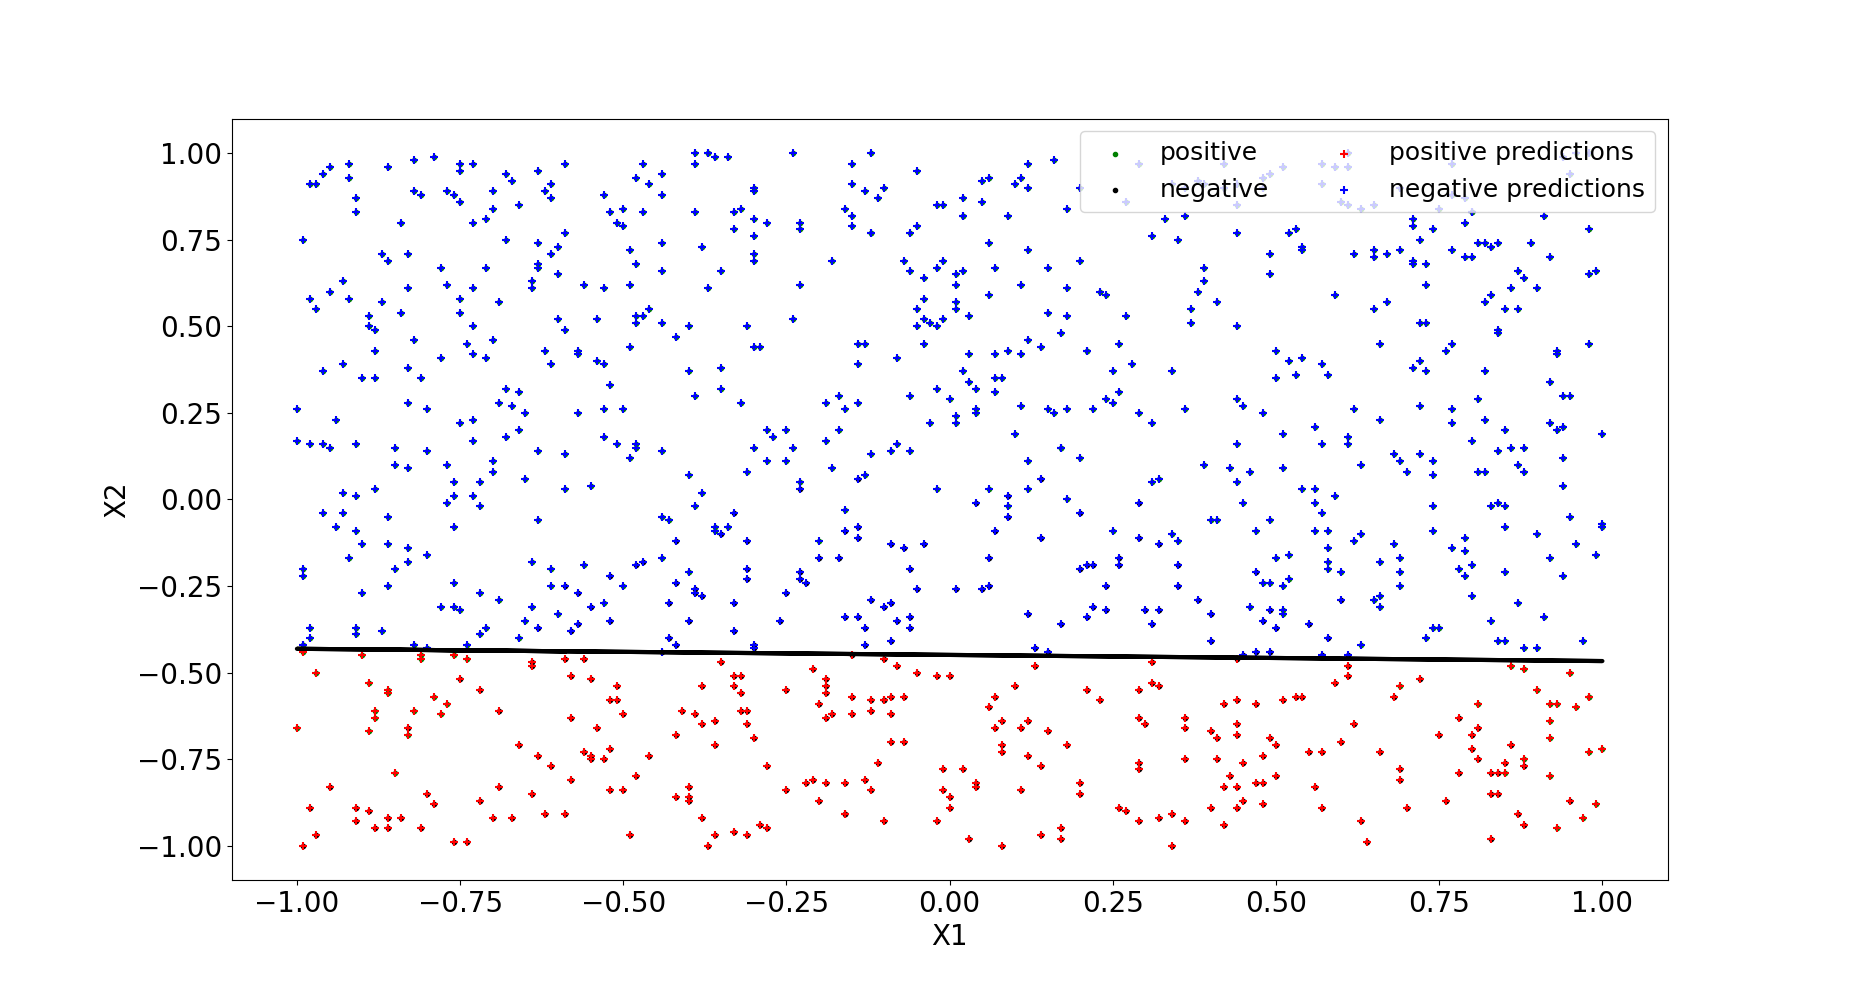
\includegraphics[scale=0.245]{Figure_C_0001.png}

C = 1

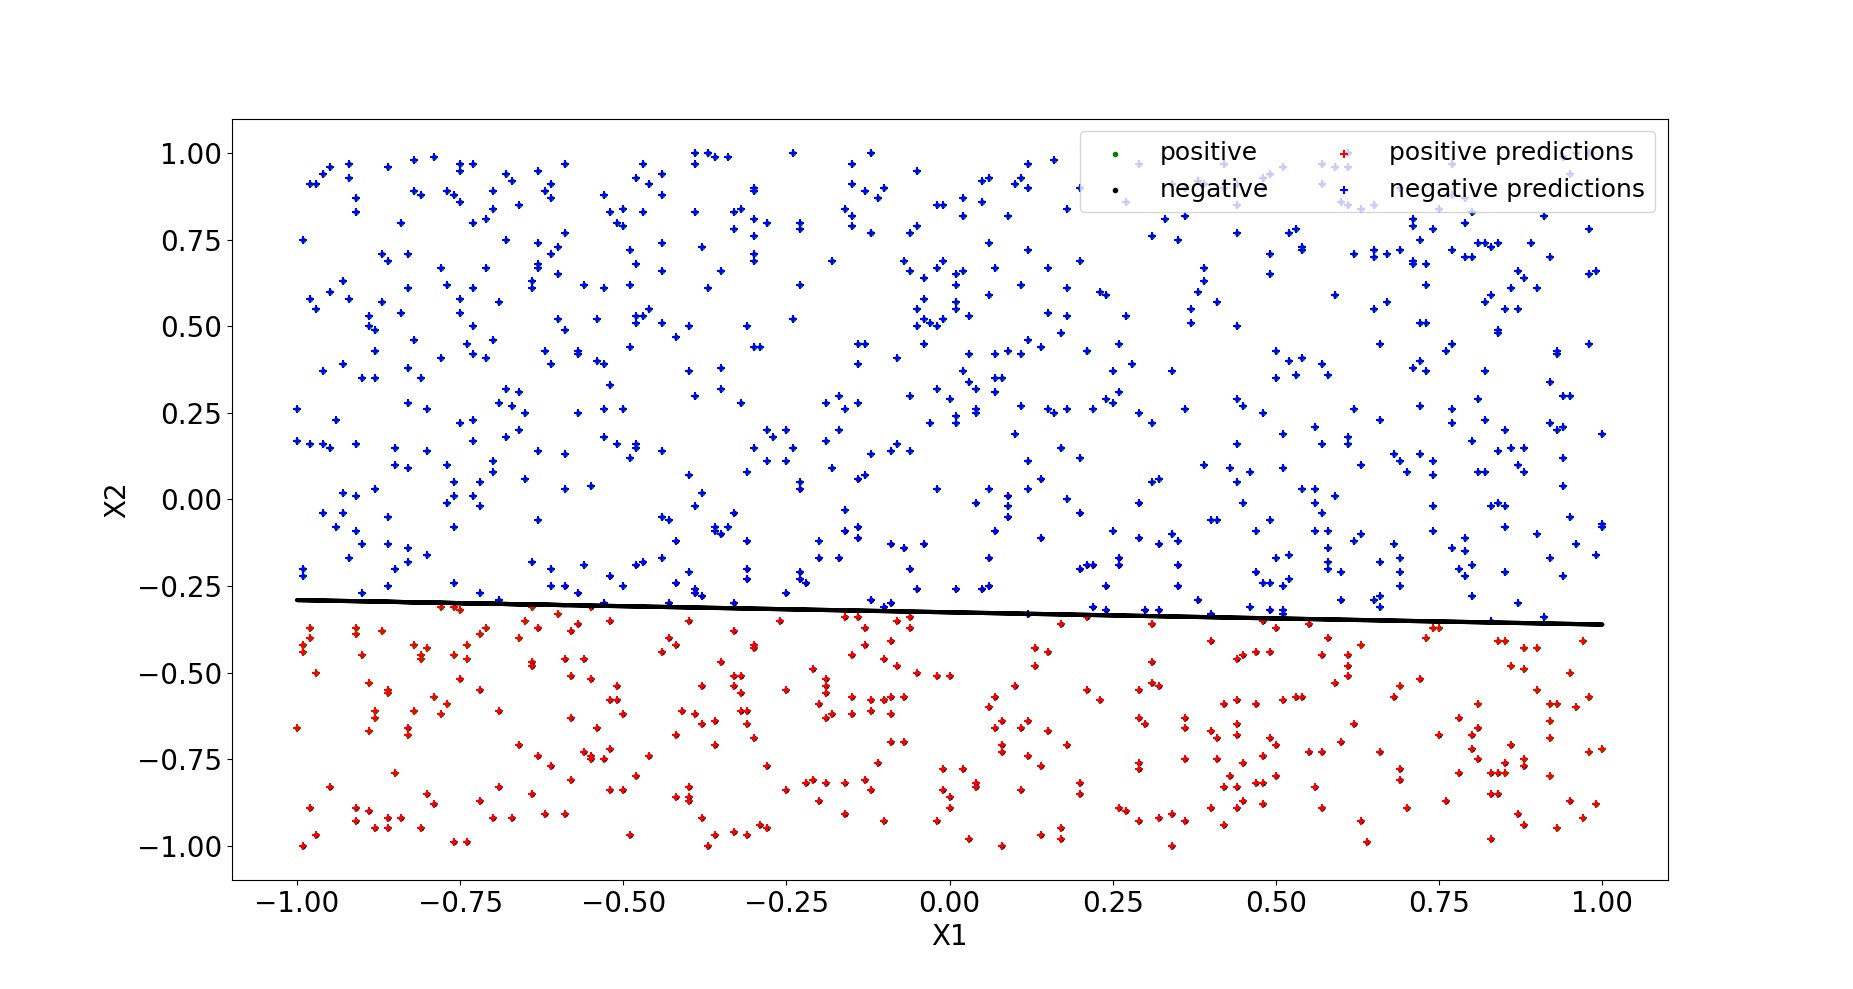
\includegraphics[scale=0.245]{Figure_C_1.png}


C = 1000

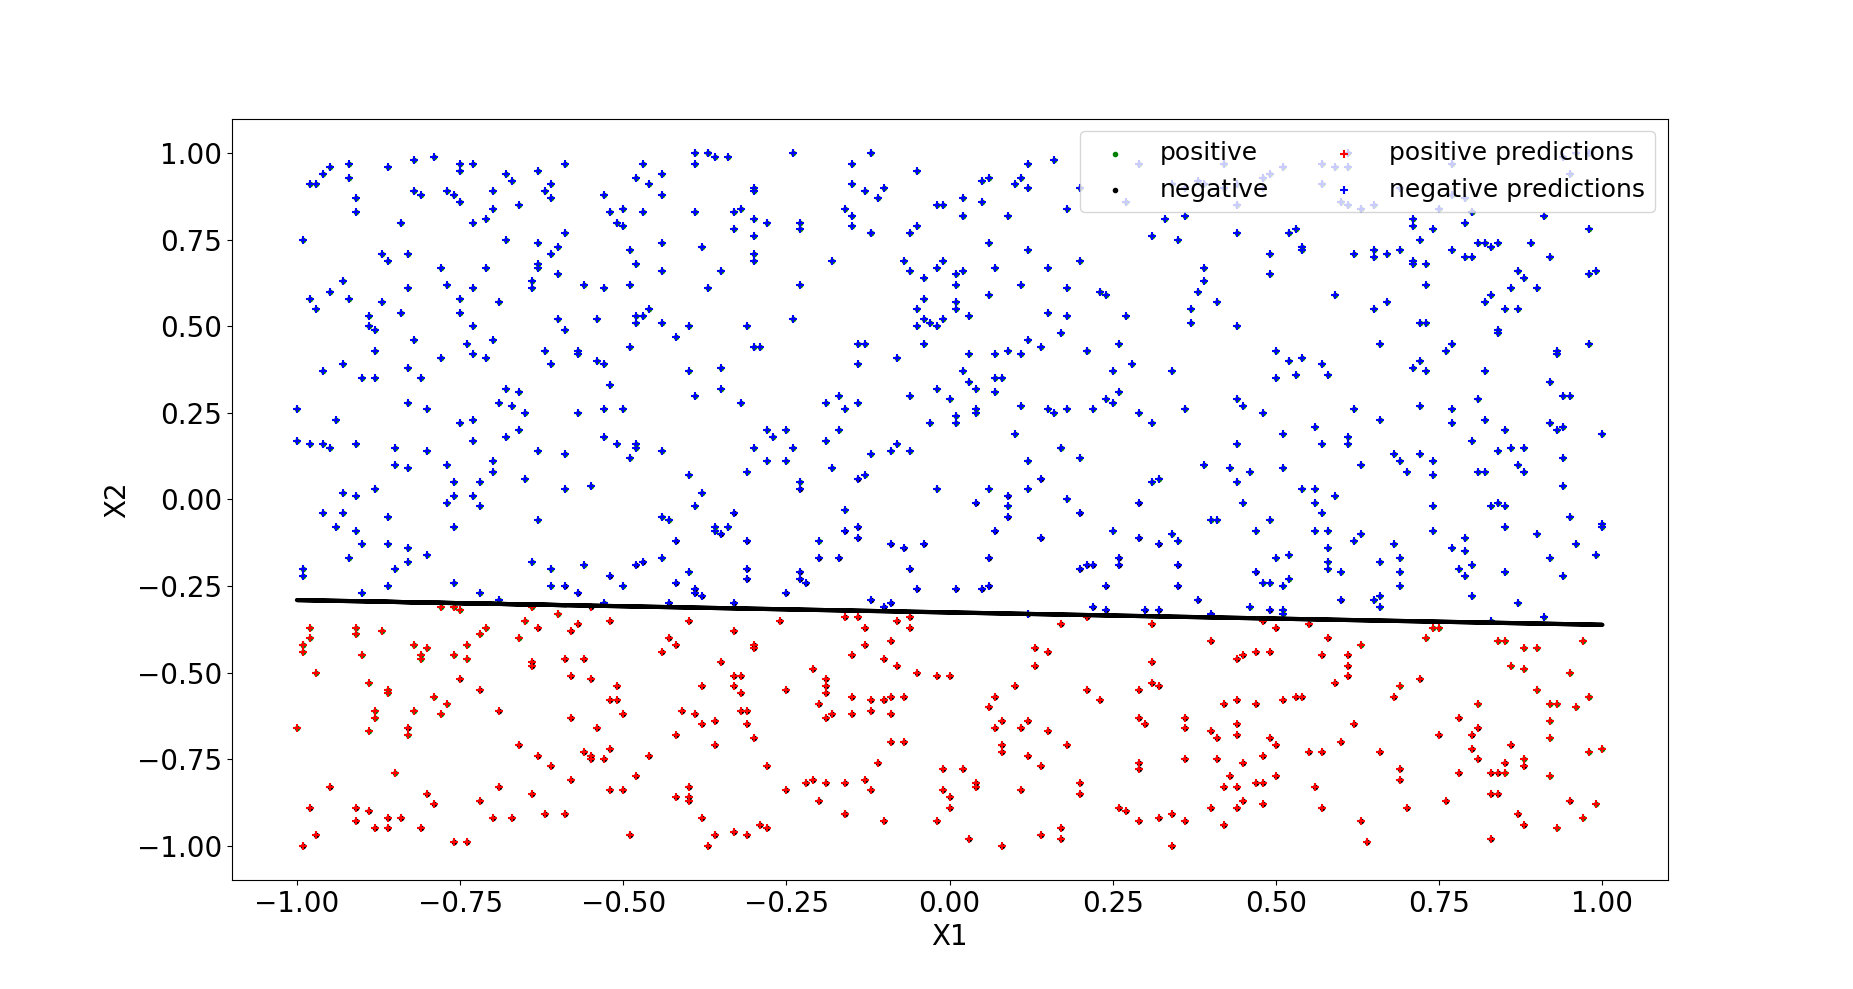
\includegraphics[scale=0.245]{Figure_C_1000.png}

\subsection*{Part iii}
A larger value for C will choose a smaller margin for the hyperplane
separating our data. In this case this results in a higher intercept value
and smaller coefficient. A smaller value for C will make the margin for data separation
bigger, potentially resulting in more misclassifications.

Looking at the plot, a higher value for C makes the separating line for the predictions
higher on the y axis (representing X2), thus prediciting more values as positive (y = 1).

A lower value for C makes the separating line lower on the y axis, thus predicting less values
as positive (y = 1).

In our situation it seems that a larger value for C works best.

\section*{Appendix}
\begin{lstlisting}[language=Python]
ADD CODE AND STUFF HERE
\end{lstlisting}
\end{document}
